% !TeX root = main.tex

%\setkeys{Gin}{draft}

\section{Assignment Goals}

%\onehalfspacing
\singlespacing
\justifying 
\par
In this lab, the common source amplifier from Lab 04 was modified by applying feedback to the circuit. Specifically, negative feedback was introduced by adding a resistor from the drain of $Q_{1}$ to the gate of $Q_{1}$. This feedback served multiple purposes, including stabilizing the DC bias point, eliminating the need for a dedicated bias voltage. The effect of feedback on bandwidth and gain was observed, showing an increase in bandwidth at the expense of overall circuit gain. However, it was also noted that feedback stabilized the gain, making it dependent only on the feedback resistor and, in this case, the signal generator resistor. The ALD1105 MOSFET was used to analyze the frequency response, and LTSpice simulations were conducted to validate measurement techniques.

\begin{center}
\begin{figure}[ht]
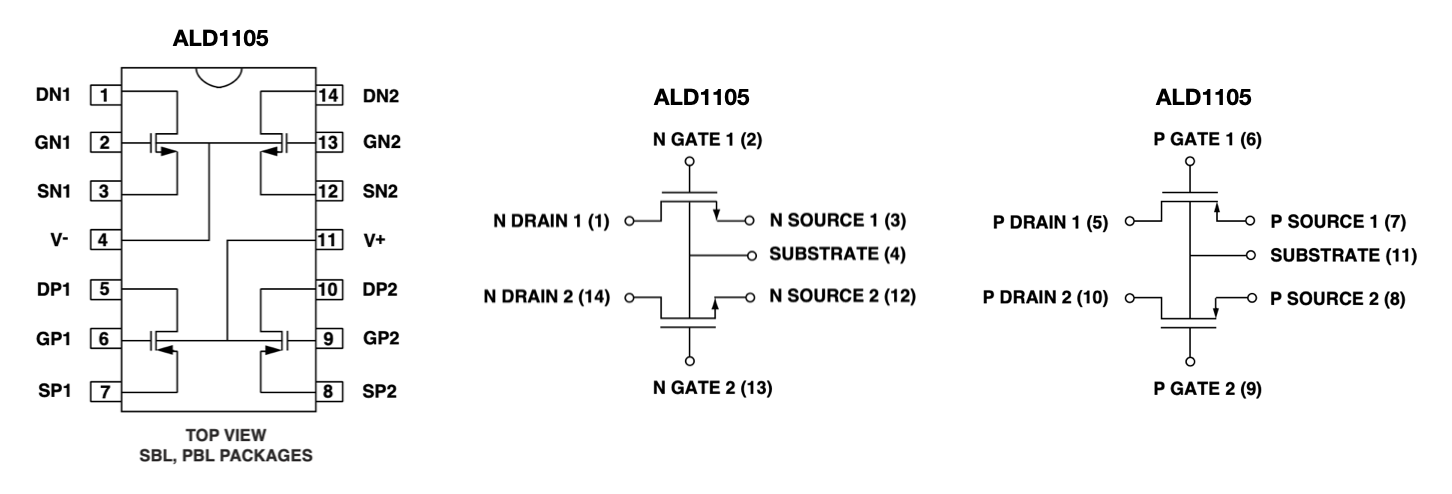
\includegraphics[scale=0.5]{Chapter_5/Lab_05_Image_1.png}
\caption{The pinout and block diagram of the ALD1105, \textbf{Note: $V^{-}$ is the body of the NMOS devices which is connected to lowest potential and $V^{+}$ is the body of the PMOS devices which is connected to the highest potential. }}
\label{fig:1}
\end{figure}
\end{center}

\section{Experiment 1: DC Operating Point}

Using the circuit shown below with the given parameter values, the potentiometer was adjusted to set the total current to $I_{Total} = 1$ mA.

\begin{itemize}

\item The DC operating point was determined by measuring the node voltages and calculating the currents. The summary table was then completed.

\end{itemize}

\begin{center}

\begin{circuitikz}[american]
\ctikzset{tripoles/mos style=arrows}

\draw

(-6,2) node[pmos,scale=2,xscale=-1] (Q3) {}
(4,2) node[pmos,scale=2] (Q2) {}
(4,-3) node[nmos,scale=2] (Q1) {}
(Q3.center) node[left] {$Q_{3}$}
(Q2.center) node[right] {$Q_{2}$}
(Q1.center) node[right] {$Q_{1}$}
(Q3.S) node[vdd] (vdd) {$+V_{DD}$}
(Q3.D) to[R=$R$] ++(0,-3) node[ground] {}
(Q3.D) to[short,*-] ++(2.5,0) to[short,-*] ++(0,1.53)
(Q3.G) -- (Q2.G)
(Q3.G) to[open,-*] ++(3,0) to[C=$C_{5}$] ++(0,2) node[ground,rotate=180] {}
(Q2.S) node[vdd] (vdd) {$+V_{DD}$}
(Q1.S) node[ground] {}
(Q2.D) -- (Q1.D)
(Q1.G)  to[short] ++(-2,0) to[C=$C_{B}$] ++(-2,0) to[R=$R_{sig}$] ++(-2,0) to[vsource,l=$v_{sig}$] ++(0,-3) node[ground] {}
(Q1.G) to[short,-*] ++(-1.5,0) to[short] ++(0,2.55) to[R=$R_{F}$] ++(3,0) to[short] ++(0.5,0) 
(Q1.G) to[short] ++(-1.5,0) to[C=$C_{1}$] ++(0,-2) node[ground] {}
(Q1.G) to[short] ++(-0.5,0) to[short,*-] ++(0,1.5) to[C,l_=$C_{2}$,-*] ++(2.45,0)
(Q2.G) to[short] ++(-0.5,0) to[short,*-] ++(0,-1.5) to[C,l=$C_{4}$,-*] ++(2.45,0)
(Q1.D) to[open] ++(0,1.5) node[left] {$V_{O}$}
(Q1.D) to[open] ++(0,1) to[C=$C_{B}$,*-] ++(3,0) to[R=$R_{L}$,v=$v_{o}$,*-] ++(0,-3) node[ground] {}
(Q1.D) to[open] ++(0,1) to[open] ++(3,0) to[short] ++(2,0) to[C=$C_{3}$] ++(0,-3) node[ground] {}
;
\end{circuitikz}

\vspace{1cm}

$V_{DD} = 10$ V \hspace{.5cm} $C_{B} = 0.022$ $\mu$F \hspace{.5cm}  $R = 25$ k$\Omega$ Potentiometer\\

\vspace{.2cm}

  $R_{F} =330$k $\Omega$ \hspace{0.5cm} $R_{sig} = 100$ k$\Omega$  \hspace{.5cm} $R_{L} =10$  M$\Omega$ (Probe)  \\

\vspace{.2cm}

$C_{1} = 10$ pF  \hspace{.5cm} $C_{2} =3.3$ pF \hspace{0.5cm} $C_{3} = 22$pF$+15$ pF (Probe)  \hspace{.5cm} $C_{4} =3.3$ pF \hspace{0.5cm} $C_{5} = 22$ pF  \\

\vspace{.5cm}
\end{center}

\section{Experiment 2: Frequency Response}
\singlespacing
Using appropriate AC measurement techniques, the frequency response of the amplifier was determined over a frequency range of 10 Hz to 100 kHz. Additionally, the following tasks were completed:

\begin{itemize}

\item The mid-band gain $\left|G_{v\text{(mid)}}\right|$ was measured.
\item The bandwidth was determined by measuring $f_{L}$ and $f_{H}$, and the Gain Bandwidth Product (GBW) was computed in Hertz. The mid-band gain was converted to V/V for accuracy.
\item The measured results were plotted against the simulated results on the same curve, using a magnitude range of 0 to +30 dB.
\item The summary tables at the end of the handout were completed.

\end{itemize}

\begin{center}


\begin{table}[H]
\begin{tabular}{ | >{\centering\arraybackslash} m{2.5cm} | >{\centering\arraybackslash} m{2.5cm} |  >{\centering\arraybackslash} m{2.5cm} | >{\centering\arraybackslash} m{2.5cm} | >{\centering\arraybackslash} m{2.5cm} |}
\hline
\multicolumn{5}{|c|}{DC Operating Point}        \\ \hline
                 Device & Quantity & Simulated  & Measured & Units \\ \hline
\multirow{5}{*}{$Q_{1}$} & $I_{D}$  & 525.197 & 500.290 & $\mu$A   \\ \cline{2-5} 
                  & $|V_{OV}|$ & 1.373 & 0.569 & V \\ \cline{2-5} 
                  &  $V_{G}$ & 1.945 & 1.142 & V  \\ \cline{2-5} 
                  & $V_{D}$ & 1.946 & 1.480 & V \\ \cline{2-5} 
                  & $V_{S}$ & 0.000 & 0.000 & V \\ \hline
                  &  &  &  &  \\ \hline
\multirow{5}{*}{$Q_{2}$} & $I_{D}$  & 525.197 & 500.290 & $\mu$A   \\ \cline{2-5} 
                  & $|V_{OV}|$ & 7.398 & 7.933 & V \\ \cline{2-5} 
                  &  $V_{G}$ & 1.956 & 1.142 & V  \\ \cline{2-5} 
                  & $V_{D}$ & 1.956 & 1.147 & V \\ \cline{2-5} 
                  & $V_{S}$ & 10.000 & 10.000 & V \\ \hline
                  &  &  &  &  \\ \hline
\multirow{5}{*}{$Q_{3}$} & $I_{D}$  & 474.798 & 500.290 & $\mu$A   \\ \cline{2-5} 
                  & $|V_{OV}|$ & 2.253 & 4.932 & V \\ \cline{2-5} 
                  &  $V_{G}$ & 7.100 & 4.421 & V  \\ \cline{2-5} 
                  & $V_{D}$ & 7.100 & 4.421 & V \\ \cline{2-5} 
                  & $V_{S}$ & 10.000 & 10.000 & V \\ \hline
\end{tabular}
\caption{DC Summary Table}
\end{table}

\newpage

\begin{table}[H]
\begin{tabular}{ | >{\centering\arraybackslash} m{3.5cm} |  >{\centering\arraybackslash} m{3cm} | >{\centering\arraybackslash} m{3cm} | >{\centering\arraybackslash} m{2cm} |}
\hline
\multicolumn{4}{|c|}{AC Summary}        \\ \hline
                 Quantity & Simulated  & Measured & Units \\ \hline
$\left|G_{v\text{(mid)}}\right|$  & 3.053  &  2.945 & V/V   \\ \cline{1-4} 
$\left|G_{v\text{(mid)}}\right|$ & 9.694  &  9.381 & dB \\ \cline{1-4} \hline
 &  &  &  \\ \hline
$f_{L}$  & 100.000 & 67.608 & Hz   \\ \cline{1-4}
$f_{H}$ & 63.100 & 138.038 & kHz \\ \cline{1-4} \hline
 &  &  &  \\ \hline
$BW$  & 137.971 & 137.971 & kHz   \\ \cline{1-4}
$GBP$ &  192.327 & 406.271 & kHz \\ \cline{1-4} \hline
\end{tabular}
\caption{AC Summary Table}
\end{table}

\end{center}

\newpage
\section{Measured Bode Plot}
\begin{center}
\begin{figure}[h]
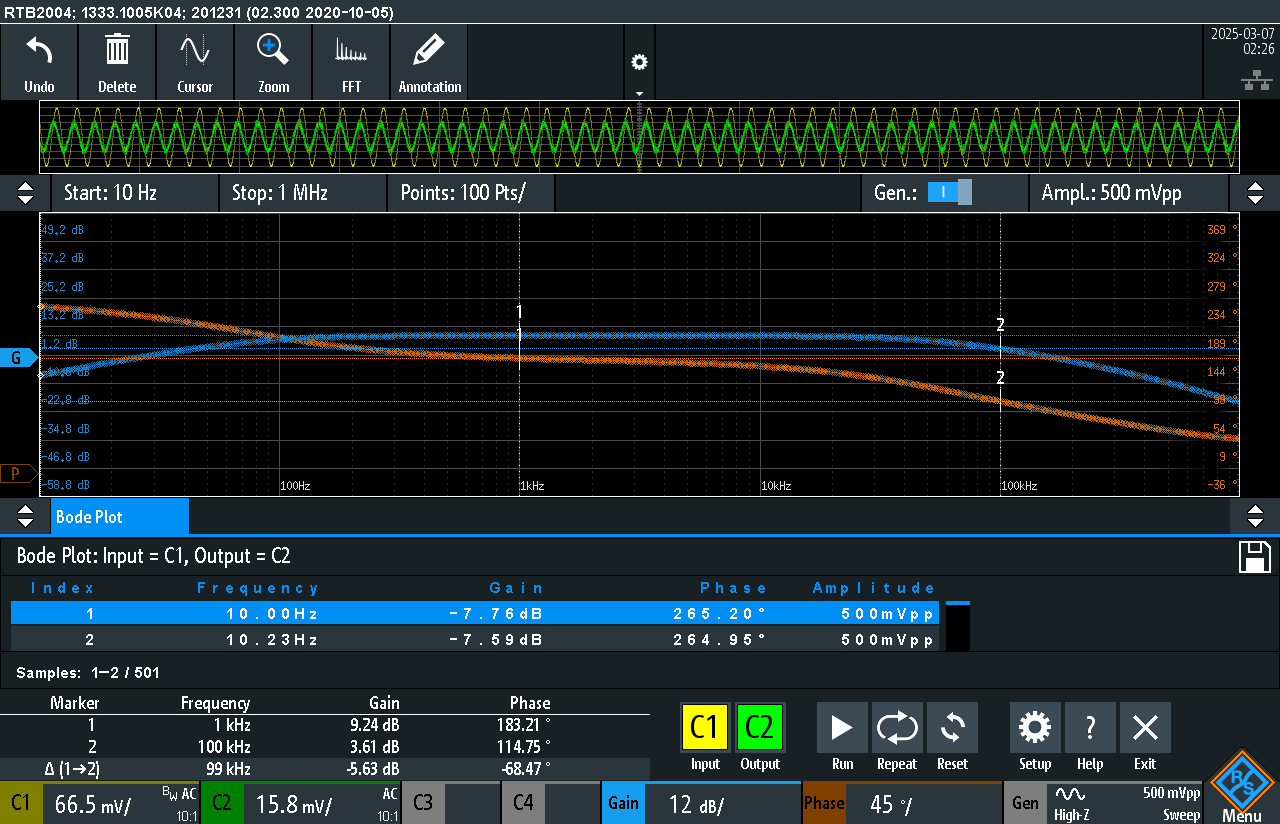
\includegraphics[scale=0.375]{Chapter_5/Lab05_Bode.png}
\caption{Measured Bode Plot of the Lab 05 circuit.}
\label{Ch5_fig:2}
\end{figure}
\end{center}

\section{Simulated vs Measured Plots}
\begin{figure}[H]
	\centering
	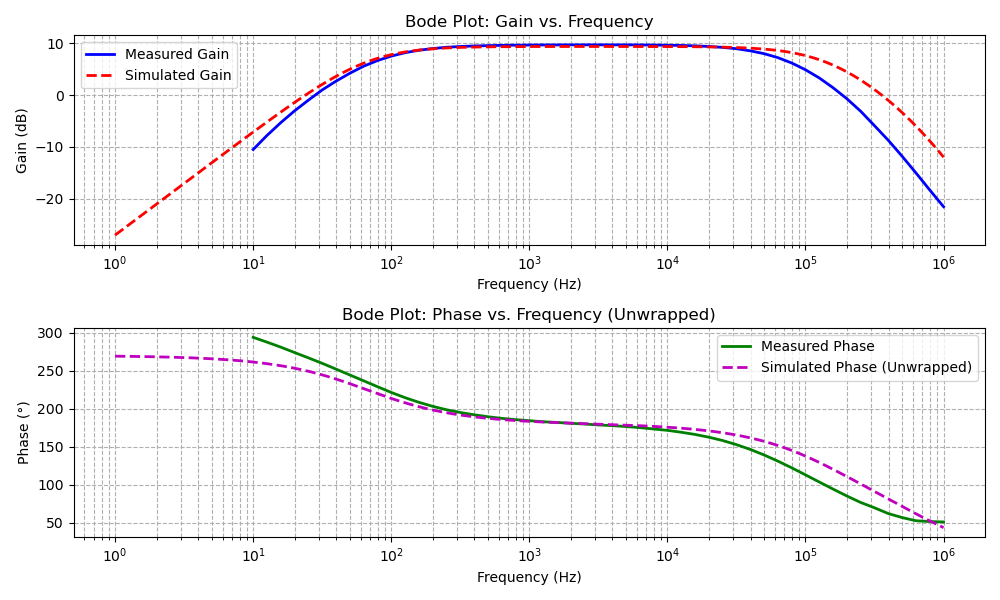
\includegraphics[width=1.0\linewidth]{Chapter_5/Lab_05_Bode_Sim_Vs_Meas_Gain_Phase.png}
	\caption{Simulated vs Measured Gain \& Phase}
	\label{Ch5_fig:3}
\end{figure}

\begin{figure}[H]
	\centering
	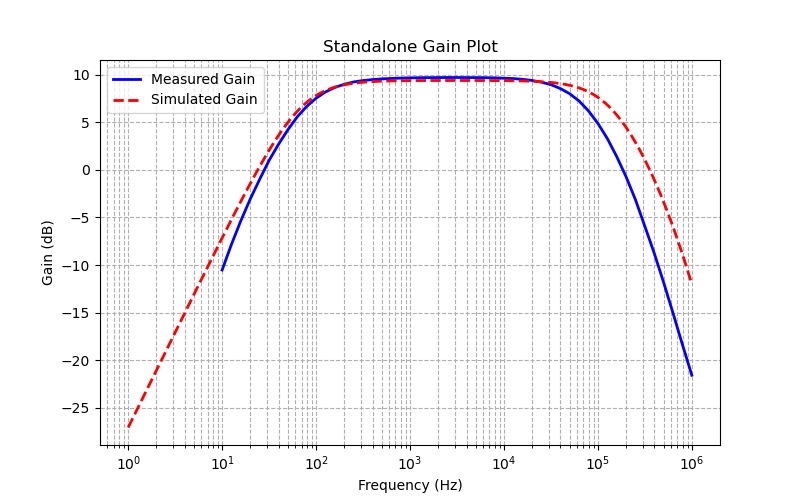
\includegraphics[width=1.0\linewidth]{Chapter_5/Lab_05_Sim_Vs_Meas_Gain.png}
	\caption{Simulated vs Measured Gain}
	\label{Ch5_fig:4}
\end{figure}

\begin{figure}[H]
	\centering
	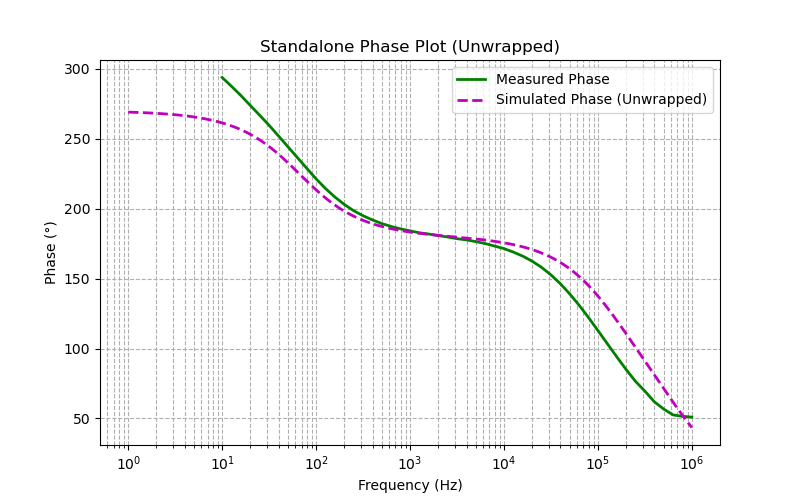
\includegraphics[width=1.0\linewidth]{Chapter_5/Lab_05_Phase_vs.png}
	\caption{Simulated vs Measured Phase}
	\label{Ch5_fig:5}
\end{figure}


\section{Python Code Listings}



\section{Conclusion}
This lab demonstrated the powerful role of negative feedback in modifying the behavior of a common source amplifier. By introducing a resistor from the drain to the gate of transistor $Q_1$​, the amplifier achieved improved DC stability without requiring a separate bias voltage. This feedback mechanism effectively stabilized the operating point and gain, making the circuit more predictable and less sensitive to parameter variations. Although the overall voltage gain was reduced, the trade-off resulted in a substantial increase in bandwidth, leading to a higher Gain-Bandwidth Product (GBW). The comparison between simulated and measured results showed good agreement, validating the effectiveness of the feedback design and confirming the accuracy of LTSpice simulations. The experiment reinforces the practical value of feedback in analog circuit design, particularly for improving linearity, stability, and frequency response.